\documentclass[12pt,oneside]{report}

%%% Load some useful packages:
%% "New" LaTeX2e graphics support.
\usepackage{graphicx}
%%	using final option to force graphics to be included even in draft mode
%\usepackage[final]{graphicx}
%% Tell graphicx the default directory for all figures
\graphicspath{{figures/}}

% Enable subfigure support
\usepackage{subfigure}

%% Make subsubsections numbered and included in ToC
\setcounter{secnumdepth}{3}
\setcounter{tocdepth}{2}

%% Package to linebreak URLs in a sane manner.
\usepackage{url}

%% Define a new 'smallurl' style for the package that will use a smaller font.
\makeatletter
\def\url@smallurlstyle{%
  \@ifundefined{selectfont}{\def\UrlFont{\sf}}{\def\UrlFont{\small\ttfamily}}}
\makeatother
%% Now actually use the newly defined style.
\urlstyle{smallurl}

%% Define 'tinyurl' style for even smaller URLs (such as in tables)
\makeatletter
\def\url@tinyurlstyle{%
  \@ifundefined{selectfont}{\def\UrlFont{\sf}}{\def\UrlFont{\scriptsize\ttfamily}}}
\makeatother

%% Provides additional functionality for tabular environments
\usepackage{array}

%% Puts space after macros, unless followed by punctuation
\usepackage{xspace}

%% Make margins less ridiculous
\usepackage{fullpage}

%% Allows insertion of fixme notes for future work
\usepackage[footnote, nomargin]{fixme}

%%%% Turned off for tech report, should be turned on for research portfolio
%% Turn on double spacing
\usepackage{setspace}
\usepackage{mdwlist}
\doublespacing

%% Make URLs clickable
%\usepackage[colorlinks, bookmarks=false]{hyperref}
\usepackage[colorlinks, bookmarks=true]{hyperref}

%% Since I'm using the LaTeX Makefile that uses dvips, I need this
%% package to make URLs break nicely
\usepackage{breakurl}

\usepackage{todonotes}
\usepackage{amsmath,amsfonts}
\numberwithin{equation}{subsection}
%%\usepackage{nonfloat}
\usepackage{bbm}
\usepackage{setspace}
\onehalfspacing
\usepackage{tabularx}

%%% End of preamble
\begin{document}

\begin{titlepage}

\begin{center}

\tiny{.}\\ [1.2cm]

\Large{Dissertation draft:} \\ [0.5cm]
\LARGE{\textsc{Software Trajectory Analysis:}} \\
\LARGE{\textsc{An empirically based method for automated software process discovery}} \\ [0.6cm]

\large{
Pavel Senin \\
Collaborative Software Development Laboratory \\
Department of Information and Computer Sciences \\
University of Hawaii \\
\texttt{senin@hawaii.edu} \\ [1.0cm]


\emph{Committee:} \\
Philip M. Johnson, Chairperson \\
%%Kyungim Baek \\
%%Guylaine Poisson \\
%%Henri Casanova \\
%%Daniel Port \\ [1.5cm]
}

\normalsize{
CSDL Technical Report 09-14 \\
\url{http://csdl.ics.hawaii.edu/techreports/09-14/09-14.pdf} \\ [1.5cm]
}

\large{2012}

\end{center}

\end{titlepage}


%% Philip suggests it needs a ToC
\tableofcontents

\begin{abstract}
%Abstract goes here if needed.
Software process defines a structure imposed on a human activity resulting in a software. 
Many different kinds of software processes were designed up today, however they are not
proven to deliver consistently and fail with equal probability. 
This phenomena was widely observed and identified as a ``software crisis'' in 1968 and 
since then it was the subject of numerous research aiming the process control and improvement. 
Today formal pocess models, standards, guidlines and recomendations provide teams 
and individuals with easy-to-understand methodologies and allow a great flexibility of 
processes for project needs, but the rate of failing software projects remains about the same. 
Recently, as an alternative opinion - the ``software development process as a craft'' 
idea emerged - this approach emphasizes roles of highly motivated, creative and skilled
individuals in software creation. Software craftsmanship paradighm of software processes 
finding  some strong supporters in the industrial and research communities recently. 

However both views, while supported by excellent research work and industrial success stories, 
follow conventional ``top-down'' technique - at first someone has to invent a
process, design and implement its building blocks and empirically evaluate it after. 
The problem with this approach, as shown in \cite{citeulike:9758924} by van der Alast,
is that one assumes an idealized versions of real processes and tend to produce 
``paper lions'' - process models which are likely to be disruptive and unacceptable for end users.

In my work I explore an alternative approach for the software process analysis - 
through the discovery of recurrent behaviors (habits) from software process artifacts trails.
Previously it was shown that it is possible to automatically recognize \cite{citeulike:2703162} 
test-driven development patterns, in my work I expand this previous experience by intoducing and 
exploring the applicability of a new temporal data mining technique in oder to find 
unknown recurrent behaviors in the space of all possible permutations of existing processes. 
Finding and understanding these recurrent behaviors may shed light on programming 
habits and their role and interactions within a software process.
\end{abstract}

% my main text chapters
\chapter{Introduction}\label{chapter_introduction}
\textit{The central issue I address in the dissertation is a possibility of recurrent behaviors discovery from 
publicly available software process artifacts by leveraging data mining and knowledge discovery techniques. 
In particular I explored an approach of discovering of recurrent behaviors through the mining of time series that
are constructed by temporal ordering of measurements extracted from software process artifacts.
Further, I shall propose a novel technique for characteristic patterns discovery from time series and show its 
applicability to the problem at hands.}

\textit{The problem's background is provided in the Section \ref{section_background}. 
Section \ref{section_software_process_design} presents classical approaches for software process design and shows its limitations.
Section \ref{section_research_hypothesis} introduces the research hypothesis.
Section \ref{knowledge_discovery} provides a background into the problem of knowledge discovery 
from time-series.
Section \ref{section_trajectory_definition} connects two problems and provides definitions.
Section \ref{section_contributions} enumerates main contributions of the thesis, 
while section \ref{section_organization} explains the thesis organization.}

%
% >> section
%
\section{Background}\label{section_background}
Contemporary software projects concern with development of complex software systems and typically have 
a considerably long life-cycle - well over decade.
A project's development and maintenance activities are usually carried out by geographically 
distributed teams and individuals. The development pace, the experience, and the structure of the 
development team continuously change with project progression and as developers joining and leaving. 
When combined with schedule and requirements adjustments, these create numerous difficulties 
for developers, users, and stakeholders, ultimately affecting the project success \cite{citeulike:2207657}. 

This software development complexity phenomena was identified in 1968 as ``Software crisis'' 
\cite{naur_crisis_68}, and was addressed by bringing the research and the practice of software development 
(or as it was called ``programming'') under the umbrella of Engineering - in an effort to provide 
the control over the process of software development. 
Following the engineering paradigm, numerous methodologies and models of software design and development 
process, known as \textit{software processes}, were proposed \cite{citeulike:10002165}.

\begin{defn}\label{def_process}
A \textbf{\textit{Software Process}} defines a sequence of activities performed in order 
to design, develop, and maintain software systems.
\end{defn}
Examples of such activities include requirements collection and creation of UML diagrams, 
requirements testing, code development,  testing, etc. The intent behind a software process is 
to provide a control over software evolution by implementing a global strategy and by structuring
and coordinating human activities in order to achieve the goal - deliver a functional software system 
on time and under the budget. 

Since then, much research has been done on software processes resulting in a number
of software development models and paradigms. Some of these were widely accepted by practitioners 
and evolved into industrial standards for software development processes such as CMM, ISO, PSP, 
and others \cite{citeulike:5043104}. However, in spite of this effort, industrial software 
development remains error-prone and more than half of all 
commercial software development projects ending up failing or being very poorly executed 
(Rubinstein, ``Chaos Reports'', 2006) \cite{chaos2006}. Some of them are abandoned due to running 
over budget, some are delivered with such low quality, or so late, that they are useless, and some, 
when delivered, are never used because they do not fulfill requirements. 

Through the analyses of software project failures, it was acknowledged, that the engineering 
paradigm might not be the best way to provide a control over software development processes 
(\cite{citeulike:3729379} \cite{citeulike:5203446}) due to the fact that Software engineering 
is dealing with significantly different from other Engineering fields problems \cite{citeulike:2207657} .
The chief argument supporting this point of view is the drastic difference in the cost model:
while in Software Engineering there is almost no cost associated with materials and 
fabrication, these usually dominate cost in all other Engineering disciplines, but, 
ironically, Software Engineering is suffering from the costs and challenges associated with 
continuous re-design of the product and its design processes - the issue which is 
hardly seen at all in other Engineering areas. 
Further, it was found, that most of the engineering-like models are rigid, ``context-free'',
and rather prescriptive, i.e. they are universally defined independently of a particular 
organizational structure or a project specificities \cite{sacchi_2001}, and while they 
structure processes and provide the control, following them does not guarantee the success.
Yet another argument supporting alternative to engineering approaches is the increasing 
understanding and appreciation of a human role in software development processes over tools, 
technologies, and standards \cite{citeulike:6580825} \cite{citeulike:149387}
\cite{1605185} \cite{citeulike:113403} \cite{1605188} \cite{citeulike:12743107}. 

Along with Software Engineering, a number of alternative, flexible and user-oriented software processes 
emerged from academy, hobbyists, and practitioners addressing aforementioned issues \cite{citeulike:3729379}. 
Among others, the Free/Libre/Open-Source Software model (FLOSS) and the software craftsmanship  
approaches gained a significant credibility in community. 
While the former \textit{holistic} software process paradigm emphasizes loosely-organized 
collaboration, frequent releases, and effectively removes the boundary between developers 
and customers, the latter, human-centric approach, is built upon the roles of highly 
motivated skilled individuals \cite{citeulike:262020} \cite{citeulike:2759198}. 

Nevertheless, alternative processes were found to be plagued by the same complexity issues. 
As it was shown, most of FLOSS projects never reach a ``magic'' 1.0 version \cite{citeulike:12480029}. 
Among others, the great "infant mortality rate" of FLOSS projects was related to a burnout, 
inability to acquire a critical mass of users, loss of leading developer(s), and forking \cite{richter2007critique}. 
Software craftsmanship, from other hands, not only challenges developers with technological advances 
requiring continuous skills improvement, but creates significant cost and effort estimation difficulties for
stakeholders and project managers \cite{citeulike:11058784}. However, despite to these issues, 
the alternative processes proved that the disciplined manner of programming and the modularization  
of the software are capable of delivering large and reliable software systems, most notable Linux OS,
suggesting that community-driven processes as good as industrial engineering-like processes.

Currently, it is widely acknowledged, that there exists no single ``silver bullet'' process which 
can bring a software development project to success \cite{citeulike:1986013}. 
Processes are numerous, each has advantages and drawbacks, and each is accompanied with 
numerous application recommendations, success stories, and with failure experiences. Nevertheless,
the alarming rate of failing projects suggests that our understanding of software process ``mechanics''  
is limited and insufficient\cite{citeulike:12550665}. 
The enormous cost of the lost effort, measured in hundreds of billions of US dollars 
\cite{citeulike:2207657} \cite{citeulike:2207653} \cite{citeulike:2207655}, 
continues to provide motivation for further research on software processes. 

%
% >> section
%
\section{Software process design}\label{section_software_process_design}
Traditionally, approaches to software process design and improvement are divided into two distinct categories. 

The first category of software process design approaches consists of traditional to engineering 
\textit{top-down} prescriptive techniques through 
\textit{proposing a process based on specific patterns of software development}. 
For example, the Waterfall Model process proposes a sequential pattern in which developers first create a 
Requirements document, then create a Design, then create an Implementation, and finally develop Tests. 
The Test Driven Development process, from other hands, proposes an iterative behavioral pattern in which
the developer must first write a test case, then write the code to implement that test case, then re-factor the 
system for maximum clarity and minimal code duplication \cite{citeulike:6086365}. 

While the top-down approach follows the usual path of trials and errors, and seems to be an extension 
of natural to humans creative processes of invention and experimentation, 
the ``invention'' of an adequate to the task software process is far from trivial 
\cite{citeulike:5043104} \cite{citeulike:1986013}. Moreover, an evaluation cycle of an invented process
is usually very expensive and considerably long.
In addition, it was shown that the process inventors are often limited in their scope and tend to assume 
idealized versions of real processes, thus, often produce ``paper lions'' - process models which are 
likely to be disruptive and unacceptable for end users, at least in their proposed form 
\cite{citeulike:9758924}, which creates a large discrepancy between actions that supposed to be done for 
the novel process and what was actually performed by particular individual or the team.

The second category of software design approaches consists of \textit{bottom-up} techniques 
that focus on a \textit{performed process reconstruction through noticing of recurrent development 
events and behaviors} or as it also called \textit{process enactment}. 
Usually, the process reconstruction task is viewed as a two-levels problem where the first level 
consists of a patterns discovery (segmentation) while the second level consists of patterns recognition 
and their network analysis \cite{citeulike:2703162}.
One of the first works in this category was by Cook and Wolf, where they show a
possibility of automated extraction of a process model through the mining of recorded 
process event logs \cite{citeulike:328044} \cite{citeulike:5120757} \cite{citeulike:5128143}. 
Later work by Huo et al. shows that it is also possible to improve an existing process
through the event logs analysis \cite{citeulike:7691059} \cite{citeulike:7690766}. 

While the bottom-up approaches seem to be more systematic and potentially less complex than invention, 
they also affected by a number of issues. A chief among these is the observability issue - 
it is usually very difficult to conduct a full depth study on a live project due to the privacy concerns. 
Moreover, it is expensive to observe a process performed by a team for a whole life-cycle of a project. 
Yet another issue is the capacity of currently available process discovery techniques - 
typically these need to be supervised by experts and finely tuned in order to reconstruct 
distributed and concurrent processes. 

Nevertheless, despite to their differences, both techniques for software process design are 
producing process models that effectively are the series of actions that must be performed successively 
(sequentially and sometimes iteratively) in order to deliver a software. 
In order to produce the viable model, the ``process inventors'' put the best of their knowledge, experience,
creativity, and logical reasoning into the proposed sequence of steps, while ``process re-constructors 
strive to eliminate the noise and to converge to a concise process model that is supported by the 
majority of observations. 
This attention to synthesis of sequential steps, leaves other phenomenas, such as team's structure, work schedule, 
developer's discipline, their behaviors, and motivation behind. While this issue was recognized previously
and resulted in a number of studies which called for attention of human element in software production 
\cite{citeulike:149387} \cite{citeulike:113403} \cite{citeulike:205322} \cite{citeulike:12798652}, 
it is still largely ignored in industrial practices \cite{citeulike:12798659}, mostly due to the 
difficulties in benefit estimation \cite{citeulike:12798662} \cite{csdl2-12-11}.

%
% >> section
%
\section{Free/Libre Open Source processes}\label{floss_processes}
Along with growing amount of publicly available software, it became obvious, that self-organizing communities of 
mostly ``recreational'' software developers and active users are capable to successfully manage large code base, 
but to deliver software increasingly complex and surprisingly popular.
Many of large, ``global'' open source software development projects, such as Linux and its derivatives, 
Gnome, Apache HTTP Server, MySQL, and others, not only have comparable with industrial projects development team 
and code-base sizes, but the same average defect rate \cite{coverity2012}. 
These facts have attracted a considerable attention from industry and many organizations 
seek to emulate successful open source software processes in traditional ``closed source'' environment 
\cite{oss_virtual_organizations} \cite{oss_balance} \cite{oss_hp} \cite{oss_4industry}. 

\begin{figure}[ht!]
   \centering
   \includegraphics[width=140mm]{figures/Linus.Kernel.ps}
   \caption{A Torvald's response suggesting that practical reasons, the ``real-life'', should be always considered 
   over specifications.
   Excerpt from the Linux mailing list. \url{http://lkml.indiana.edu/hypermail/linux/kernel/0509.3/1441.html}}
   \label{fig:kernel}
\end{figure}

If we consider this as an assertion that open-source software processes are at least as good as engineering-like 
software process models, then, the freely available open-source process software artifacts potentially bear an 
incredible wealth of the information worth of studying. Moreover, the striking differences of open-source processes 
from a traditional software development could potentially reveal novel software processes and their aspects that 
were previously not accounted for. 
For example, consider that the most significant document in industrial software processes - a specification - 
is rarely considered at all in open source world. In FLOSS projects the software look and its functionality are 
rather viewed as open-end questions. Even in the Linux kernel development, which is probably one of the few strictly 
moderated FLOSS development processes, developers prise practical reasons over specifications 
\ref{fig:kernel}.

Yet another source of motivation for studying of public FLOSS software process artifacts comes from the fact that 
in order to facilitate the distributed FLOSS software development processes, the community is highly encouraging
developers to commit their changes rather often \cite{so-checkin} \cite{git-best-practices1}.
The frequent commits and the changes visibility practice is often cited as vital for health of software 
process as mentioned in some lengthy discussions: ``\textit{Don't Go Dark}'' \cite{checkin-dgd-2008}, 
``\textit{Check In Early, Check In Often}'' \cite{checkin-ch-2012}. Potentially, frequent commits create artifacts 
trails that provide finer resolution into project development and allow more thorough process recovery.

%
% >> section
%
\section{Public software repositories}\label{section_public_repositories}
Recently, the aforementioned situation changed, and the interest for process enactment and reconstruction, 
as well as attention to the human-specific components of software processes has been revived. 
This change is driven by the increase in public data that are made available by the proliferation of open 
source communities.

Currently, with accessible personal computers, friendly software development toolkits, and due to massification
of the use of the web as
a platform for collaborative work, small-scale commercial and recreational 
programming become very popular. 
Today, free code hosting sites such as SourceForge, GoggleCode, and GitHub host thousands of 
Free/Libre Open Source Software (FLOSS) projects.
These publicly offer numerous software artifacts such as design documents, source codes, bugs and issue records, and 
developers and users communications.
Further, Q\&A and social websites for developers such as StackOverflow, Biostars, TopCoder and others becoming 
increasingly popular among the software developers as places for exchanging experiences, learning new tricks, and 
improving skills, plus, they offer anonymized data back to the community.

The public availability of numerous software process artifacts effectively removes not only the high cost of observation, 
but most of the privacy concerns - the two issues that previously made any large-scale analysis of software projects 
unfeasible for most researchers.

Scientific community response on the availability of public artifacts was overwhelming, and a number of 
venues was established addressing the increased interest. 
Since 2004, the International Conference on Software Engineering (ICSE) hosts a Working Conference on 
Mining Software Repositories (MSR). The original call for papers stated MSR's purpose as 
\textit{``... to use the data stored in these software repositories to further understanding of software 
development practices ... [and enable repositories to be] used by researchers to gain empirically based 
understanding of software development, and by software practitioners to predict and plan various aspects 
of their project''} \cite{msr2004} \cite{citeulike:7853299}. 
Several other venues: International Conference on Predictive Models in Software Engineering \cite{promise12}, 
International Conference on Open Source Systems, the Workshop on Public Data about Software Development, 
and the International Workshop on Emerging Trends in FLOSS Research have also played
an important role in shaping and advancing this research domain.

Some of the published work addresses the software process discovery. Among others, most notable and 
relevant to my research is work by Jensen \& Scacchi. In their early work, they demonstrated, that 
information reflecting software processes can be gathered from public systems \cite{citeulike:12550640}. 
Later, in \cite{citeulike:5043664} and \cite{citeulike:5128808}, they show, that by manual mapping of 
collected process evidence to a pre-defined process meta-model it is possible to reconstruct some 
of the FLOSS processes. 
Another closely related to my research is work by Hindle et al. where they has shown that it is possible to 
discover software process evidence through partitioning \cite{citeulike:10377366}.

However, the research work based on mining of software process artifacts shows, that while public availability 
of artifacts is minimizing observability and privacy issues, the nature of these artifacts creates a number of 
challenges which I discuss in the chapter X, which limit the possible scope of the research and significantly 
elevate the complexity of the process discovery effectively rendering previously designed techniques inefficient.
Thus, the novel analysis and discovery techniques are needed to be developed for public software process artifacts 
analysis \cite{citeulike:7853299}.
% when ``\textit{... going beyond code and bugs...}'' 

%
% >> section
%
\section{Research hypothesis, scope of the dissertation}\label{section_research_hypothesis}
In previous sections, I have outlined the evidence of a limited performance of existing engineering-like 
software processes (Section \ref{section_background}),
as well the oversight of a variety of human factors that fall beyond a typical sequence of development 
actions by traditional approaches to software process design (Section \ref{section_software_process_design}).
Then, I have identified a few differences of FLOSS processes from traditional Software Engineering 
(Section \ref{floss_processes}), which can potentially shed light on human-driven aspects of software development.
Finally, I have pointed out a growing wealth of publicly available software process artifacts 
(Section \ref{section_public_repositories}) that is worth to explore for a better understanding not only 
FLOSS software processes, but their human factors. All this provided a motivation to my exploratory study, 
whose details I outline in this section.

In my work, I attempted to explore the possibility of discovery of a specific human-driven aspect in 
FLOSS software development that is a \textit{\textbf{behavior}}, which I define as the mannerism in which a 
developer, or a team, conduct their everyday work. 
In particular, I explore the possibility of discovery of \textit{recurrent behaviors}, i.e. behaviors supported 
by a numerous evidence, from software process artifacts. 

For example, if within an observation interval one developer frequently runs unit tests before committing 
changes into repository, while another usually commit changes without running the tests, the first developer's
habit of testing a code before the commit is a recurrent behavior that may reflect the developer's discipline,
or an unusual attention to some particular part of the code. 
Consider another example, if one of the developers usually commits code changes in mornings, while another 
developer late in the day, these two recurrent behaviors, might indicate a constraints that are put on the 
project, or the process, or on the developers themselves.
Obviously, latter behaviors should be possible to quantify by simple analysis of commit timestamps, while 
the former can be discovered by the analysis of co-occurring changes in the source code. 
Moreover, these and similar recurrent behaviors could be further associated with certain project's or process 
traits, such as pace, agility, size, complexity, code quality and others, which will not only extend our 
knowledge of human factors in software processes, but will lay a foundation for future research in software 
processes.

To begin with, I hypothesized, that \textbf{\textit{it is possible to discover recurrent behaviors from 
publicly available software process artifacts}}. 

Following the hypothesis, I have investigated a number of publicly available software repositories,
their artifacts, and a number of applicable data-mining techniques in a preliminary exploratory study 
\cite{csdl2-10-09}. However, similarly to other studies in the field, I have discovered, that while FLOSS 
process artifacts are numerous and readily accessible, their irregular, snapshot-like nature and the poor 
informational content significantly limit the applicability of known techniques for process mining.

In order to overcome this issue, I have casted the initial problem of event-based recurrent behaviors 
discovery into more generic problem of knowledge discovery from time series and approached it
by developing a novel technique for interpretable comparative analysis of time series that allows 
characteristic patterns discovery and ranking called SAX-VSM \cite{sax-vsm}. 

Further, I have developed a software artifacts analysis framework, called Software Trajectory Analysis, 
which aids in software artifacts collection, software process and product evolutionary metrics extraction, 
and their comparative analyses that enable discovery and ranking of characteristic patterns.


 in rank highlight is  transformation into  and by using I approached the problem of knowledge discovery 

developed a 
software process artifacts mining framework called Software Trajectory Analysis which is built upon 
a novel technique for comparative analysis of time series that allows characteristic patterns discovery 
and ranking.

This dissertation presents its results, as well as introduces a novel data mining technique designed to 
alleviate difficulties with interpretability of quantitative results obtained through mining of software
artifacts trails. 

%
% >> section
%
\section{Knowledge discovery from time series}\label{section_knowledge_discovery}
In data mining, time series are used as a proxy representing a vast variety of real-life phenomena 
in wide range of fields including, but not limited to physics, medicine, meteorology, 
music, motion capture, image recognition, signal processing, and text mining. 
While time series usually directly represent observed phenomenas by capturing their measurable evolution in time, 
the pseudo time series often used for representation of various high-dimensional data 
by combining data points into ordered sequences. 
For example in spectrography data values are ordered by component wavelengths \cite{citeulike:12550833};
in shape analysis the order is the clockwise walk direction starting from a
specific point in the outline \cite{citeulike:12550835}, in image classification the numbers of pixels
are sorted by color component values \cite{citeulike:2900542}.

Many important problems of knowledge discovery from time series reduce to the core task of finding 
characteristic, likely to be repeated, sub-sequences in a longer time series. 
In the early work these were called as 
\textit{frequent patterns} \cite{citeulike:5159615}, 
\textit{approximate periodic patterns} \cite{citeulike:1959582},
\textit{primitive shapes} \cite{citeulike:5898869}, 
\textit{class prototypes} \cite{citeulike:4406444}, 
or \textit{understandable patterns} \cite{citeulike:3978076}. 
Later, similarly to Bioinformatics, these were unified under the term \textit{motif} \cite{citeulike:3977965}.
Once found, motifs can be used for a hypothesis generation by finding their associations with known,
or unknown phenomenas \cite{citeulike:3977965}. 

The recent advances in semi-supervised and unsupervised finding of such characteristic sub-sequences, 
in particular work based on \textit{shapelets} \cite{citeulike:7344347} \cite{citeulike:11957982}
\cite{citeulike:12552293} and \textit{bag of patterns} \cite{citeulike:10525778}, show a great potential 
of application of time series data-mining techniques to a wide variety of high-dimensional data.

Unfortunately, both techniques provide a limited insight into the data and suffer from performance issues. 
While exact shapelet techniques allow discovery of class-characteristic patterns and facilitate classification,
algorithm is almost quadratic and provides limited insight into class specificities. 
The bag of patterns algorithm, while performs in a linear time, requires a previous knowledge for input parameters 
selection and does not offer class generalization.

In order to overcome this limitations, in this thesis I propose a novel approach for time-series classification and 
knowledge discovery that is called SAX-VSM and is based on symbolic approximation of time series and vector space model. 
As I shall show, SAX-VSM is capable to discover and to rank characteristic subsequences representing time series classes. 
The proposed algorithm not only facilitates classification, but provides insights into the both: classification results 
and time series classes specificities. As I shall show, by facilitating the class' characteristics patterns ranking,
SAX-VSM enables the discovery of recurrent behaviors and their heat-map like visualization. 

\section{Software trajectory analysis}\label{section_trajectory_definition}
Previously, Johnson et al. defined \textit{software metrics telemetry streams} \cite{citeulike:12550871}, 
(what they re?) and showed, that it is possible to improve software development process by using the 
knowledge extracted by experts through visual analysis of these streams.
 
Similarly to software metrics telemetry streams, I abstract software process artifact by collecting their 
metrics and arrange these measurements by artifact creation time into high-dimensional vectors. 
These non-equidistant, often sparse and uneven in length time series 
I call ``\textbf{software trajectories}''. Similarly to approximate trajectories of objects in 
a physical space, or reduced in complexity sequence of states of a dynamic system (Poincare' maps), 
the \textit{software trajectory is a curve that describes a software project progression in a space 
of a chosen metrics}.

Through an exploratory study, I have discovered, that by the comparative analysis of software trajectories 
with SAX-VSM it is possible to discover and to interpret recurrent behaviors. This workflow that 
consists of software artifacts collection, their metrics extraction, and comparative analyses I call 
\textit{\textbf{Software Trajectory Analysis}} (STA). 

In this thesis, through three case studies, I will show, that Software Trajectory Analysis is capable 
of discovering of a various characteristic patterns which ca be associated with recurrent behaviors.

\section{Contributions}\label{section_contributions}
Main contributions of my work can be summarized as follows: 
\begin{itemize}
\item I propose a novel, generic algorithm for interpretable time series classification: SAX-VSM. 
While the classification performance of this algorithm is at the level of current state of the art, 
it offers an outstanding feature - discovery, generalization, and ranking of class-characteristic features. 
This, in turn, enables knowledge discovery by offering much clearer insight into classification results than any of 
competing techniques.
In addition, SAX-VSM is very fast in classification and has a small memory footprint. 
Overall, I expect this algorithm to play an important role in future because of the growing ubiquity of time series and 
a growing interest in behaviors.
\item Powered by SAX-VSM, I design a Software Trajectory Analysis (STA) framework, and through case-studies 
show its capacity for recurrent behaviors discovery from publicly available software process
artifacts. While case studies are obviously limited, I argue that STA is a useful knowledge discovery tool applicable for a 
variety of software process artifacts and metrics. 
\item Finally, I provide SAX-VSM and STA implementations to community.
\end{itemize}

\section{Dissertation Outline}\label{section_organization}
The rest of this dissertation is organized as follows. Chapter \ref{chapter_background_work} discusses the history 
of Software Engineering, previous work in software process discovery, mining of software repositories, and current 
state of the art in time series mining. Chapter \ref{chapter_sax_vsm} proposes an algorithm for interpretable 
time series classification. Chapter \ref{chapter_sta} discusses the design of STA framework and presents case studies.
Chapter \ref{chapter_conclusions} concludes and discusses several directions for future study.
\section{Software Process}
The Institute of Electrical and Electronics Engineers defines software engineering as 
“the application of a systematic, disciplined, quantifiable approach to development, 
operation, and maintenance of software; that is, the application of engineering software”

\chapter{Process Modeling}
\chapter{Process Mining}

\section{Software Process Recovery}
Software development process was always being under focus of various stakeholders due to the number of reasons ranging from standards compliance to business and security intelligence. When no live observations are made on the performers, due to the availability, timing, cost, or privacy issues, recovering software process from artifacts could be complex and expensive process. Researchers have suggested a possibility of software process recovery by interviewing of developers and managers and by analysis of process artifacts: such as printed documents - designs, use-cases, software inspections or electronic artifact trails: version, bug and issue control systems and mailing lists. This research resulted in many published work:
\begin{itemize}
\item{Cook \& Wolf in \cite{citeulike:328044} discuss an event-based framework for process discovery based on grammar inference and finite state machines. The authors directly applied their framework to Software Configuration Management (SCM) logs demonstrating satisfactory results.}
\item{Jensen \& Scacchi \cite{citeulike:5043664} describe an interesting framework built upon mapping between process artifacts and process entities into an universal generic meta-model. Application of their human-involved technique leveraged a pre-existing domain knowledge for the effective pruning and iterative process revision resulted in ``workflows discovery''.}
\item{German in \cite{citeulike:421438} performed a manual mining of the GNOME process artifacts: documentations, CVS logs, and one hundred and four mailing-lists in order to
describe the development processes from GSD (Global Software Development) point of view.}
\item{Ripoche tried a more automatic approach in \cite{citeulike:9112798} by developing a generic model for process-based explanation of bugs persistence using state diagrams and
probabilistic choices.}
\end{itemize}
All these suggests that software process artifacts bear enough information about performed process for its recontsruction. In my study I havily relying on this fact. This not only serves as a foundation of my hypothesis, but also partially assures the validity of my approach to the software process reconstruction. Further in this chapter I will introduce a novel technique of pattern mining form the software process artifacts trails. After introduction of the technique, I will walk through the performed case studies in which I have applied this technique to the various types of the software process artifact trails.

\subsection{Apriori algorithm}

Family of seminal Apriori algorithms was proposed in 1994 by Agrawal \& Srikant \cite{citeulike:775528}. These algorithms are based on the naive \textit{apriori association rule} stating that \textit{any sub-pattern of a frequent pattern must be frequent}. The name ``apriori'' is based on the fact of using of a prior knowledge by the algorithm: the $k$-th itemsets are used to generate $(k+1)$ itemsets.

Algorithm starts by scanning a database and finding all possible $1$-itemsets counting their support and keeping only those which satisfy to the minimal support value. This itemsets result in the set $L_{1}$. This set, in turn, is used to construct $L_{2}$ set which is a combination of all possible itemsets from $L_{1}$, once construction of $L_{2}$ complete one full scan of the database required to compute the support of each of the itemsets. For finding the $L_{3}$ and so on the Apriori property is used, which reduces the search space while generating candidates. Apriori property is that \textit{all non-empty subsets of the frequent itemset must be also frequent}.

The apriori property is used in the candidate itemset generation step in the next fashion: if itemset $I$ does not satisfies to minimal support value, i.e. $Support(I) \; \leq \; min\_support$, the itemset $I'$ resulting from adding item $i$ into the $I$ ($I' = I \cup i$) cannot occur mor efrequently than $I$, i.e. $Support(I') \; \leq \; min\_support$. In some literature this property called \textit{antimonotone} property as an opposite to monotone one.

The generation of itemsets $L_{k}$ for $k > 2$ consists of two steps: join and prune.

\textbf{The Join step.}

To find itemset $L_{k}$ based on $L_{k-1}$ we first generate the set $C_{k}$ - the set of all candidate patterns based on the join of $L_{k-1}$ with itself: $L_{k-1} \times L_{k-1}$. We will introduce a notation $l_{i,j}$ for $j$th item of the itemset $i$, also we must note, that by convention, Apriori assumes that all items within an itemset $l_{i}$ are sorted alphabetically, i.e. that $l_{i,j} < l_{i,j+1}$. Taking all above in the account, the join of $L_{k-1} \times L_{k-1}$ is performed only on itemsets $l_{i}$ and $l_{j}$ if their first $k-2$ items are the same, i.e. $l_{i,m} = l_{j,m}, \; \forall m \in [0,k-2]$, this generates next candidate itemsets: ${l_{i,1},l_{i,2},l_{i,3},...,l_{i,k-1},l_{j,k-1}}$. Here we are also making sure that $l_{i,k-1} < l_{j,k-1}$ to avoid duplicates within $C_{k}$.

\textbf{The Prune step.}

The set $C_{k}$ generated during the join step is a superset of $L_{k}$ and it's members may not be frequent enough to satisfy a minimal support value.


\section{Symbolic Aggregate approXimation (SAX)} \label{sax}
\begin{figure}[tbp]
   \centering
   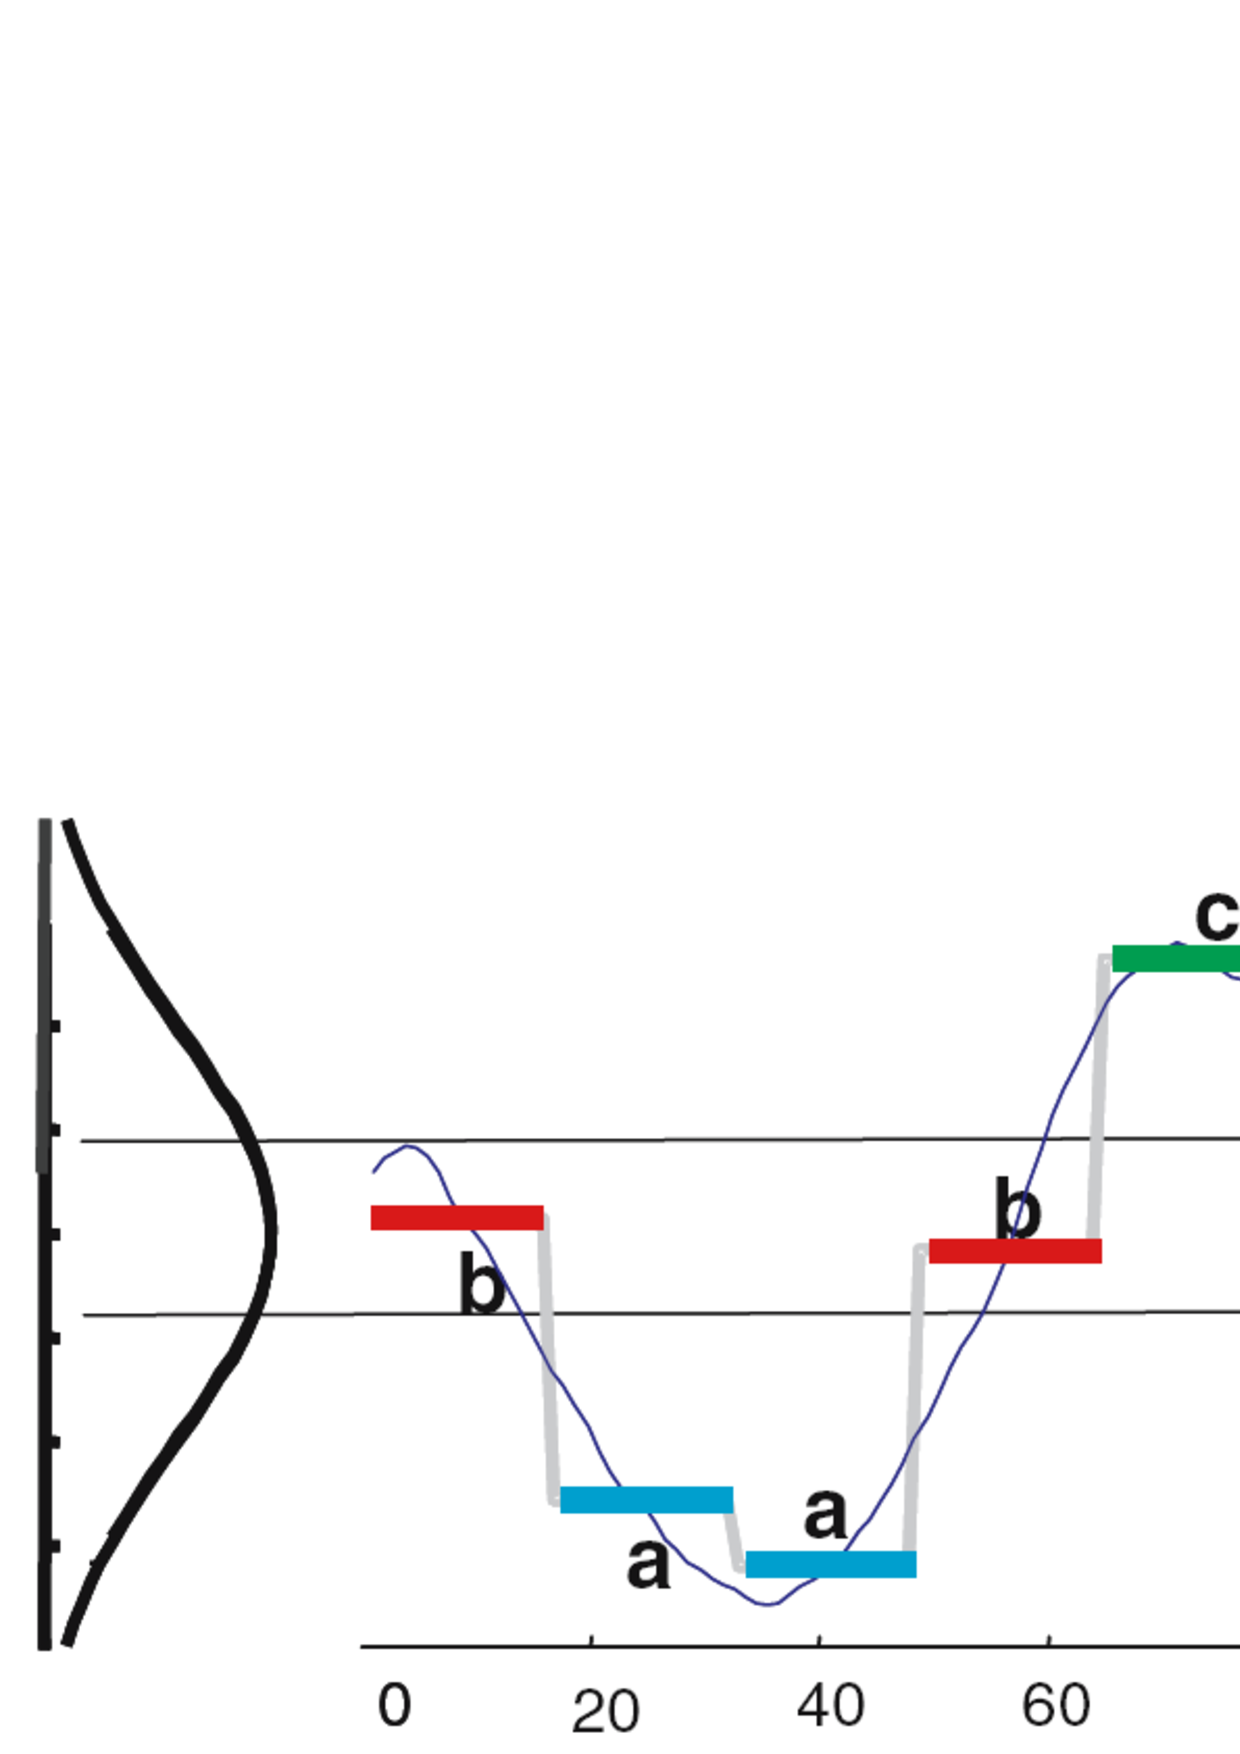
\includegraphics[height=45mm]{sax_intro}
   \caption{The illustration of the SAX approach taken from \cite{citeulike:2821475} depicts two pre-determined breakpoints for the three-symbols alphabet and the conversion of the time-series of length $n=128$ into PAA representation followed by mapping of the PAA coefficients into SAX symbols with $w=8$ and $a=3$ resulting in the string \textbf{baabccbc}.}
   \label{fig:sax_intro}
\end{figure}

Symbolic Aggregate approXimation was proposed by Lin et al. in \cite{citeulike:2821475}. This method extends the PAA-based approach \cite{citeulike:2946589} \cite{citeulike:3000416}, inheriting algorithmic simplicity and low computational complexity, while providing satisfiable sensitivity and selectivity in range-query processing. Moreover, the use of a symbolic representation opens the door to the existing wealth of data-structures and string-manipulation algorithms in computer science such as hashing, regular expression pattern matching, suffix trees etc.

SAX transforms a time-series $X$ of length $n$ into a string of arbitrary length $\omega$, where $\omega << n$ typically, using an alphabet $A$ of size $ a \geq 2$. The SAX algorithm consist of two steps: during the first step it transforms the original time-series into a PAA representation and this intermediate representation gets converted into a string during the second step. Use of PAA at the first step brings the advantage of a simple and efficient dimensionality reduction while providing the important lower bounding property as shown in the previous section. The second step, actual conversion of PAA coefficients into letters, is also computationally efficient and the contractive property of symbolic distance was proven by Lin et al. in \cite{citeulike:532335}.

\begin{equation}
D_{PAA}(\bar{X}, \bar{Y}) \equiv \sqrt{\frac{n}{M}} \sqrt{ \sum_{i=1}^{M} 
\left(  \bar{x}_{i} - \bar{y}_{i} \right)}
\label{eq:paa_distance}
\end{equation}

Discretization of the PAA representation of a time-series into SAX is implemented in a way which produces symbols corresponding to the time-series features with equal probability. The extensive and rigorous analysis of various time-series datasets available to the authors has shown that normalized by the zero mean and unit of energy time-series follow the Normal distribution law. By using Gaussian distribution properties, it's easy to pick $a$ equal-sized areas under the Normal curve using  lookup tables  \cite{citeulike:4434481} for the cut lines coordinates, slicing the under-the-Gaussian-curve area. 
The $x$ coordinates of these lines called ``breakpoints'' in the SAX algorithm context. The list of breakpoints $B=\beta_{1}, \beta_{2}, ... , \beta_{a-1}$ such that $\beta_{i-1} < \beta_{i}$ and $\beta_{0} = -\infty$, $\beta_{a} = \infty$ divides the area under $N(0,1)$ into $a$ equal areas. By assigning a corresponding alphabet symbol $alpha_{j}$ to each interval $[\beta_{j-1},\beta_{j})$, the conversion of the vector of PAA coefficients $\bar{C}$ into the string $\hat{C}$ implemented as follows:
\begin{equation}
\hat{c}_{i} = alpha_{j}, \; \text{iif} \; \bar{c}_{i} \in [\beta_{j-1},\beta_{j})
\label{eq:alpha}
\end{equation}

\begin{figure}[tbp]
   \centering
   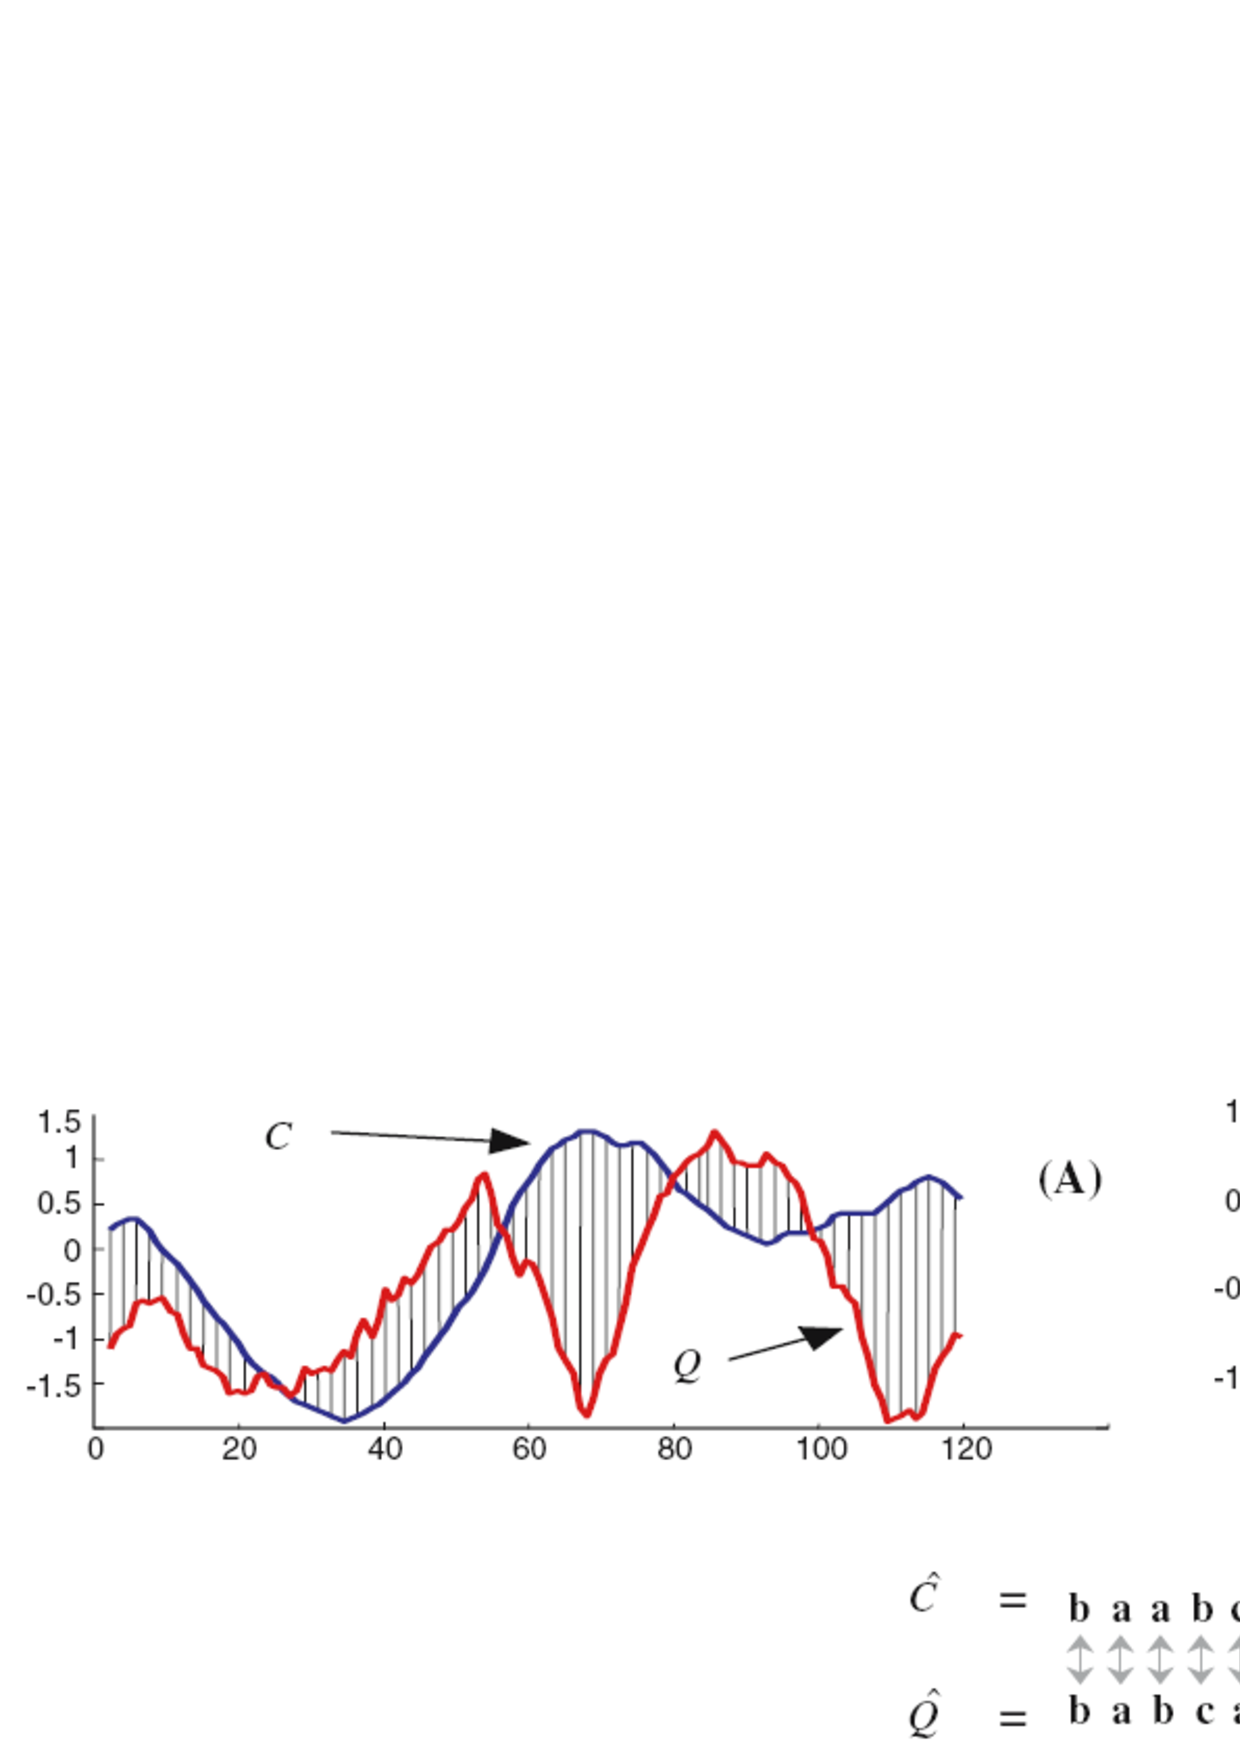
\includegraphics[height=47mm]{sax_distance}
   \caption{The visual representation of the two time-series $Q$ and $C$ and three distances between their representation: Euclidean distance between raw time-series (A), the distance defined for PAA coefficients (B) and the distance between two SAX representations (C). (The figure taken from \cite{citeulike:2821475} as well)}
   \label{fig:sax_distance}
\end{figure}

SAX introduces new metrics for measuring distance between strings by extending Euclidean and PAA (\ref{eq:paa_distance}) distances. The function returning the minimal distance between two string representations of original time series $\hat{Q}$ and $\hat{C}$ is defined as
\begin{equation}
MINDIST(\hat{Q},\hat{C}) \equiv \sqrt{ \frac{n}{w} } \sqrt{ \sum_{i=1}^{w} ( dist( \hat{q}_{i}, \hat{c}_{i} ) )^{2}}
\label{eq:sax_mindist}
\end{equation} 
where the $dist$ function is implemented by using the lookup table for the particular set of the breakpoints (alphabet size) as shown in Table \ref{tbl:sax_lookup}, and where the singular value for each cell $(r,c)$ is computed as 
\begin{equation}
cell_{(r,c)} = 
\begin{cases} 
0, \text{ if }\left| r-c \right| \leq 1 \\
\beta_{\max(r,c) - 1} - \beta_{\min(r,c) - 1}, \text{ otherwise}
\end{cases}
\label{eq:cell}
\end{equation}

\begin{table}
\begin{tabularx}{400pt}{X X X X X}
\hline
   & a   & b    & c    & d    \\
\hline
a & 0    & 0    & 0.67 & 1.34 \\
b & 0    & 0    & 0    & 0.67 \\
c & 0.67 & 0    & 0    & 0    \\
d & 1.34 & 0.67 & 0    & 0    \\
\hline
\end{tabularx}
\caption{A lookup table used by the MINDIST function for the $a=4$}
\label{tbl:sax_lookup}
\end{table}

As shown by Li et al., this SAX distance metrics lower-bounds the PAA distance, i.e.
\begin{equation}
\sum_{i=1}^{n} (q_{i} - c_{i})^{2} \geq n(\bar{Q} - \bar{C})^{2} \geq n(dist(\hat{Q},\hat{C}))^2
\label{eq:sax_bounding}
\end{equation}

The SAX lower bound was examined by Ding et al. \cite{citeulike:4501572} in great detail and found to be superior in precision to the spectral decomposition methods on bursty (non-periodic) data sets.



\chapter{Getting Data}

\section{Software configuration management}
Software evolve. The software evolution happens under the pressure from stakeholders, end users and due to the infomation technology evolution. It is practically inevitable.
\todo[size=\tiny]{Here I need to narrow the need of SCM and the evolution of software}
``Software configuration management'' or SCM (also known as ``software change and configuration management'') is a term used to descibe means of software evolution control by
software developers. These include but no limited to standards, approaches, techniques and tools for initiating, evaluating, and controlling change of software product before,
during and after the development process. Configuration management is an integral part of the software process spanning across all its phases and providing stucture and control
imposed on the software change, thus enabling it to be performed in a way which is reproducible and does not destroy the integrity of software.

Recalling the discussion of Goals of SCM will clearly paint a picture of what basic features an ideal SCM Tool should have in it.
•       First and most basic functionality a Software Configuration Management tool should provide is support for a central file repository. All other functionalities are around
managing and tracking of these repository items.
•       Secondly it is important that the SCM tool provides the capabilities of the distributed team to work together from a central repository. Features like file locking
mechanism, file comparison and atomic commits are to name a few.
•       The SCM tool should also provide a simple mechanism for creating and maintaining private branches and for merging changes from the main code line to the private branch, and
vice versa.
•       The SCM tool should provide visibility into changes made for each task and support the ability to work by task instead of by individual file, to merge changes from one
configuration to another, and to revert changes for a task if needed.
•       The SCM tool should also provide an easy mechanism for rolling back to the last good integration version.
•       The SCM tool supports simple creation of a hierarchy, give visibility into the changes at each stage, and enable straightforward merging between stages.
•       Tagging is another feature very common and useful which involves giving meaningful names to specific revisions. These names are generally called Tags or Labels.
•       The SCM tool should support re-targeting features without the need to write and maintain scripts to perform the operations.
•       In order to re-factor code and still be able to trace through the history of changes, an SCM tool must support file and directory rename and move operations and track the
operations as part of the element’s history.
•       The SCM tool should easily integrate with the continuous integration server so that latest code from the SCM repository can be extracted and compiled continuously and whole
process can be automated.


\chapter{Software Process Discovery}
\section{Software process recovery from SCM system}
As Ball et al. \cite{citeulike:9004378} and Zimmermann \& WeiBgerber
\cite{citeulike:5058462} point out - all of the contemporary version control
systems provide considerably large amount of auxiliary information about
software change. In particular, version control system, when coupled with a
mailing lists and (or) bug and issue tracking system is capable of providing
information \textit{who} changed \textit{what} and \textit{why}. Which seems to
be a fair amount of information needed for one's opinion about the change. It is
possible to get an overall understanding of the change necessity through the
analysis of bug and issue reports. Version control itself provides quantitative
data about files and LOC and changed, added or deleted. The analysis of code
snapshots (versions) allows to quantify the change in terms of various software
metrics like complexity, cohesion etc. When considered in time all this data
provides a solid background for a software evolution research.

However, what is very difficult to know from any contemporary SCM system is that
a software process behind the changes. Nevertheless many research in the field
of MSR was done in order to shed a light on the software process itself.
\cite{citeulike:9007622} There are only traces of such information present in
version control transactions. In order to recover some insights about the
performed software process information behind a software change statistics
behind the change can show us some behavioral patterns blanks in the single
transactions can be restored by statistics
outliers effect can be diminished by statistics


\chapter{Case Studies}

\chapter{Conclusions}
The ultimate premise of STA is to provide means for empirical guidance of developers and project 
management in software process execution and decision-making improvement.


%%% Input file for bibliography
\bibliography{seninp}
%% Use this for an alphabetically organized bibliography
\bibliographystyle{plain}
%% Use this for a reference order organized bibliography
%\bibliographystyle{unsrt}
%% Try using this BibTeX style that hopefully will print annotations in
%% the bibliography. This will allow me to make notes on papers in the
%% BibTeX file and have them readable in the references section until
%% I turn them into a conceptual literature review 
%\bibliographystyle{annotation}

\end{document}
